%===============================================================================
% LaTeX sjabloon voor de bachelorproef toegepaste informatica aan HOGENT
% Meer info op https://github.com/HoGentTIN/latex-hogent-report
%===============================================================================

\documentclass[dutch,dit,thesis]{hogentreport}

% TODO:
% - If necessary, replace the option `dit`' with your own department!
%   Valid entries are dbo, dbt, dgz, dit, dlo, dog, dsa, soa
% - If you write your thesis in English (remark: only possible after getting
%   explicit approval!), remove the option "dutch," or replace with "english".

\usepackage{lipsum} % For blind text, can be removed after adding actual content

%% Pictures to include in the text can be put in the graphics/ folder
\graphicspath{{graphics/}}

%% For source code highlighting, requires pygments to be installed
%% Compile with the -shell-escape flag!
\usepackage[section]{minted}
%% If you compile with the make_thesis.{bat,sh} script, use the following
%% import instead:
%% \usepackage[section,outputdir=../output]{minted}
\usemintedstyle{solarized-light}
\definecolor{bg}{RGB}{253,246,227} %% Set the background color of the codeframe

%% Change this line to edit the line numbering style:
\renewcommand{\theFancyVerbLine}{\ttfamily\scriptsize\arabic{FancyVerbLine}}

%% Macro definition to load external java source files with \javacode{filename}:
\newmintedfile[javacode]{java}{
    bgcolor=bg,
    fontfamily=tt,
    linenos=true,
    numberblanklines=true,
    numbersep=5pt,
    gobble=0,
    framesep=2mm,
    funcnamehighlighting=true,
    tabsize=4,
    obeytabs=false,
    breaklines=true,
    mathescape=false
    samepage=false,
    showspaces=false,
    showtabs =false,
    texcl=false,
}

% Other packages not already included can be imported here

%%---------- Document metadata -------------------------------------------------
% TODO: Replace this with your own information
\author{Ernst Aarden}
\supervisor{Dhr. F. Van Houte}
\cosupervisor{Mevr. S. Beeckman}
\title[Optionele ondertitel]%
    {Titel van de bachelorproef}
\academicyear{\advance\year by -1 \the\year--\advance\year by 1 \the\year}
\examperiod{1}
\degreesought{\IfLanguageName{dutch}{Professionele bachelor in de toegepaste informatica}{Bachelor of applied computer science}}
\partialthesis{false} %% To display 'in partial fulfilment'
%\institution{Internshipcompany BVBA.}

%% Add global exceptions to the hyphenation here
\hyphenation{back-slash}

%% The bibliography (style and settings are  found in hogentthesis.cls)
\addbibresource{bachproef.bib}            %% Bibliography file
\addbibresource{../voorstel/voorstel.bib} %% Bibliography research proposal
\defbibheading{bibempty}{}

%% Prevent empty pages for right-handed chapter starts in twoside mode
\renewcommand{\cleardoublepage}{\clearpage}

\renewcommand{\arraystretch}{1.2}

%% Content starts here.
\begin{document}

%---------- Front matter -------------------------------------------------------

\frontmatter

\hypersetup{pageanchor=false} %% Disable page numbering references
%% Render a Dutch outer title page if the main language is English
\IfLanguageName{english}{%
    %% If necessary, information can be changed here
    \degreesought{Professionele Bachelor toegepaste informatica}%
    \begin{otherlanguage}{dutch}%
       \maketitle%
    \end{otherlanguage}%
}{}

%% Generates title page content
\maketitle
\hypersetup{pageanchor=true}

%%=============================================================================
%% Voorwoord
%%=============================================================================

\chapter*{\IfLanguageName{dutch}{Woord vooraf}{Preface}}%
\label{ch:voorwoord}

%% TODO:
%% Het voorwoord is het enige deel van de bachelorproef waar je vanuit je
%% eigen standpunt (``ik-vorm'') mag schrijven. Je kan hier bv. motiveren
%% waarom jij het onderwerp wil bespreken.
%% Vergeet ook niet te bedanken wie je geholpen/gesteund/... heeft

\lipsum[1-2]
%%=============================================================================
%% Samenvatting
%%=============================================================================

% TODO: De "abstract" of samenvatting is een kernachtige (~ 1 blz. voor een
% thesis) synthese van het document.
%
% Een goede abstract biedt een kernachtig antwoord op volgende vragen:
%
% 1. Waarover gaat de bachelorproef?
% 2. Waarom heb je er over geschreven?
% 3. Hoe heb je het onderzoek uitgevoerd?
% 4. Wat waren de resultaten? Wat blijkt uit je onderzoek?
% 5. Wat betekenen je resultaten? Wat is de relevantie voor het werkveld?
%
% Daarom bestaat een abstract uit volgende componenten:
%
% - inleiding + kaderen thema
% - probleemstelling
% - (centrale) onderzoeksvraag
% - onderzoeksdoelstelling
% - methodologie
% - resultaten (beperk tot de belangrijkste, relevant voor de onderzoeksvraag)
% - conclusies, aanbevelingen, beperkingen
%
% LET OP! Een samenvatting is GEEN voorwoord!

%%---------- Nederlandse samenvatting -----------------------------------------
%
% TODO: Als je je bachelorproef in het Engels schrijft, moet je eerst een
% Nederlandse samenvatting invoegen. Haal daarvoor onderstaande code uit
% commentaar.
% Wie zijn bachelorproef in het Nederlands schrijft, kan dit negeren, de inhoud
% wordt niet in het document ingevoegd.

\IfLanguageName{english}{%
\selectlanguage{dutch}
\chapter*{Samenvatting}
\lipsum[1-4]
\selectlanguage{english}
}{}

%%---------- Samenvatting -----------------------------------------------------
% De samenvatting in de hoofdtaal van het document

\chapter*{\IfLanguageName{dutch}{Samenvatting}{Abstract}}

   Deze bachelorproef onderzoekt de optimalisatie van educatief gebruik: beperking en flexibele activering van E-commerce Platforms en sociale media in de scholengroep IÑIGO. Ook vergelijkt het welke methode de balans tussen gebruiksgemak, algemene kosten en functionaliteiten voor het beheren van toegang tot E-commerce en sociale media platforms in het onderwijs vormt, met als doel de afleiding te minimaliseren en educatief gebruik te optimaliseren. De motivatie voor dit onderzoek ligt in de groeiende uitdagingen waarmee het onderwijs geconfronteerd wordt bij het beheren van een gebalanceerde en gecontroleerde toegang tot E-commerce en sociale media platforms.\newline
   
   De probleemstelling richt zich voornamelijk op de vraag hoe scholen de toegang tot E-commerce en sociale media op een efficiënte manier kunnen beheren, zodat leerlingen niet afgeleid worden en tegelijkertijd de voordelen van deze platforms kunnen verwerken tijdens de lessen. De hoofdvraag van het onderzoek is: Welke methode vormt de balans tussen gebruiksgemak, algemene kosten en functionaliteiten voor het beheren van toegang tot E-commerce en sociale media platforms in het onderwijs, met als doel de afleiding te minimaliseren en educatief gebruik te optimaliseren?\newline
   
   Een uitgebreide literatuurstudie waarin de vergelijking van verschillende softwareoplossingen wordt gemaakt, biedt een antwoord op de hoofdvraag. Op basis van de resultaten uit de literatuurstudie is de meest veelbelovende softwareoplossing geïmplementeerd, getest en uitgewerkt in de proof of concept. \newline
   
   Uit het onderzoek blijkt dat de geteste softwareoplossing echter niet volledig voldeed aan de gestelde criteria en de vereisten van de casus. Hieruit kan geconcludeerd worden dat er meer onderzoek naar passende methode nodig is om centraal beheer van de websites aan te tonen, zodat leerlingen flexibele toegang hebben tot websites die niet van toepassing zijn tijdens de schooluren.

   
   
   
   

%---------- Inhoud, lijst figuren, ... -----------------------------------------

\tableofcontents

% In a list of figures, the complete caption will be included. To prevent this,
% ALWAYS add a short description in the caption!
%
%  \caption[short description]{elaborate description}
%
% If you do, only the short description will be used in the list of figures

\listoffigures

% If you included tables and/or source code listings, uncomment the appropriate
% lines.
%\listoftables
%\listoflistings

% Als je een lijst van afkortingen of termen wil toevoegen, dan hoort die
% hier thuis. Gebruik bijvoorbeeld de ``glossaries'' package.
% https://www.overleaf.com/learn/latex/Glossaries

%---------- Kern ---------------------------------------------------------------

\mainmatter{}

% De eerste hoofdstukken van een bachelorproef zijn meestal een inleiding op
% het onderwerp, literatuurstudie en verantwoording methodologie.
% Aarzel niet om een meer beschrijvende titel aan deze hoofdstukken te geven of
% om bijvoorbeeld de inleiding en/of stand van zaken over meerdere hoofdstukken
% te verspreiden!

%%=============================================================================
%% Inleiding
%%=============================================================================

\chapter{\IfLanguageName{dutch}{Inleiding}{Introduction}}%
\label{ch:inleiding}

De inleiding moet de lezer net genoeg informatie verschaffen om het onderwerp te begrijpen en in te zien waarom de onderzoeksvraag de moeite waard is om te onderzoeken. In de inleiding ga je literatuurverwijzingen beperken, zodat de tekst vlot leesbaar blijft. Je kan de inleiding verder onderverdelen in secties als dit de tekst verduidelijkt. Zaken die aan bod kunnen komen in de inleiding~\autocite{Pollefliet2011}:

\begin{itemize}
  \item context, achtergrond
  \item afbakenen van het onderwerp
  \item verantwoording van het onderwerp, methodologie
  \item probleemstelling
  \item onderzoeksdoelstelling
  \item onderzoeksvraag
  \item \ldots
\end{itemize}

\section{\IfLanguageName{dutch}{Probleemstelling}{Problem Statement}}%
\label{sec:probleemstelling}

Uit je probleemstelling moet duidelijk zijn dat je onderzoek een meerwaarde heeft voor een concrete doelgroep. De doelgroep moet goed gedefinieerd en afgelijnd zijn. Doelgroepen als ``bedrijven,'' ``KMO's'', systeembeheerders, enz.~zijn nog te vaag. Als je een lijstje kan maken van de personen/organisaties die een meerwaarde zullen vinden in deze bachelorproef (dit is eigenlijk je steekproefkader), dan is dat een indicatie dat de doelgroep goed gedefinieerd is. Dit kan een enkel bedrijf zijn of zelfs één persoon (je co-promotor/opdrachtgever).

\section{\IfLanguageName{dutch}{Onderzoeksvraag}{Research question}}%
\label{sec:onderzoeksvraag}

Wees zo concreet mogelijk bij het formuleren van je onderzoeksvraag. Een onderzoeksvraag is trouwens iets waar nog niemand op dit moment een antwoord heeft (voor zover je kan nagaan). Het opzoeken van bestaande informatie (bv. ``welke tools bestaan er voor deze toepassing?'') is dus geen onderzoeksvraag. Je kan de onderzoeksvraag verder specifiëren in deelvragen. Bv.~als je onderzoek gaat over performantiemetingen, dan 

\section{\IfLanguageName{dutch}{Onderzoeksdoelstelling}{Research objective}}%
\label{sec:onderzoeksdoelstelling}

Wat is het beoogde resultaat van je bachelorproef? Wat zijn de criteria voor succes? Beschrijf die zo concreet mogelijk. Gaat het bv.\ om een proof-of-concept, een prototype, een verslag met aanbevelingen, een vergelijkende studie, enz.

\section{\IfLanguageName{dutch}{Opzet van deze bachelorproef}{Structure of this bachelor thesis}}%
\label{sec:opzet-bachelorproef}

% Het is gebruikelijk aan het einde van de inleiding een overzicht te
% geven van de opbouw van de rest van de tekst. Deze sectie bevat al een aanzet
% die je kan aanvullen/aanpassen in functie van je eigen tekst.

De rest van deze bachelorproef is als volgt opgebouwd:

In Hoofdstuk~\ref{ch:stand-van-zaken} wordt een overzicht gegeven van de stand van zaken binnen het onderzoeksdomein, op basis van een literatuurstudie.

In Hoofdstuk~\ref{ch:methodologie} wordt de methodologie toegelicht en worden de gebruikte onderzoekstechnieken besproken om een antwoord te kunnen formuleren op de onderzoeksvragen.

% TODO: Vul hier aan voor je eigen hoofstukken, één of twee zinnen per hoofdstuk

In Hoofdstuk~\ref{ch:conclusie}, tenslotte, wordt de conclusie gegeven en een antwoord geformuleerd op de onderzoeksvragen. Daarbij wordt ook een aanzet gegeven voor toekomstig onderzoek binnen dit domein.
\chapter{\IfLanguageName{dutch}{Stand van zaken}{State of the art}}%
\label{ch:stand-van-zaken}

% Tip: Begin elk hoofdstuk met een paragraaf inleiding die beschrijft hoe
% dit hoofdstuk past binnen het geheel van de bachelorproef. Geef in het
% bijzonder aan wat de link is met het vorige en volgende hoofdstuk.

% Pas na deze inleidende paragraaf komt de eerste sectiehoofding.

Dit hoofdstuk bevat je literatuurstudie. De inhoud gaat verder op de inleiding, maar zal het onderwerp van de bachelorproef *diepgaand* uitspitten. De bedoeling is dat de lezer na lezing van dit hoofdstuk helemaal op de hoogte is van de huidige stand van zaken (state-of-the-art) in het onderzoeksdomein. Iemand die niet vertrouwd is met het onderwerp, weet nu voldoende om de rest van het verhaal te kunnen volgen, zonder dat die er nog andere informatie moet over opzoeken \autocite{Pollefliet2011}.

Je verwijst bij elke bewering die je doet, vakterm die je introduceert, enz.\ naar je bronnen. In \LaTeX{} kan dat met het commando \texttt{$\backslash${textcite\{\}}} of \texttt{$\backslash${autocite\{\}}}. Als argument van het commando geef je de ``sleutel'' van een ``record'' in een bibliografische databank in het Bib\LaTeX{}-formaat (een tekstbestand). Als je expliciet naar de auteur verwijst in de zin (narratieve referentie), gebruik je \texttt{$\backslash${}textcite\{\}}. Soms is de auteursnaam niet expliciet een onderdeel van de zin, dan gebruik je \texttt{$\backslash${}autocite\{\}} (referentie tussen haakjes). Dit gebruik je bv.~bij een citaat, of om in het bijschrift van een overgenomen afbeelding, broncode, tabel, enz. te verwijzen naar de bron. In de volgende paragraaf een voorbeeld van elk.

\textcite{Knuth1998} schreef een van de standaardwerken over sorteer- en zoekalgoritmen. Experten zijn het erover eens dat cloud computing een interessante opportuniteit vormen, zowel voor gebruikers als voor dienstverleners op vlak van informatietechnologie~\autocite{Creeger2009}.

Let er ook op: het \texttt{cite}-commando voor de punt, dus binnen de zin. Je verwijst meteen naar een bron in de eerste zin die erop gebaseerd is, dus niet pas op het einde van een paragraaf.

\lipsum[7-20]

%%=============================================================================
%% Methodologie
%%=============================================================================

\chapter{\IfLanguageName{dutch}{Methodologie}{Methodology}}%
\label{ch:methodologie}

%% TODO: In dit hoofstuk geef je een korte toelichting over hoe je te werk bent
%% gegaan. Verdeel je onderzoek in grote fasen, en licht in elke fase toe wat
%% de doelstelling was, welke deliverables daar uit gekomen zijn, en welke
%% onderzoeksmethoden je daarbij toegepast hebt. Verantwoord waarom je
%% op deze manier te werk gegaan bent.
%% 
%% Voorbeelden van zulke fasen zijn: literatuurstudie, opstellen van een
%% requirements-analyse, opstellen long-list (bij vergelijkende studie),
%% selectie van geschikte tools (bij vergelijkende studie, "short-list"),
%% opzetten testopstelling/PoC, uitvoeren testen en verzamelen
%% van resultaten, analyse van resultaten, ...
%%
%% !!!!! LET OP !!!!!
%%
%% Het is uitdrukkelijk NIET de bedoeling dat je het grootste deel van de corpus
%% van je bachelorproef in dit hoofstuk verwerkt! Dit hoofdstuk is eerder een
%% kort overzicht van je plan van aanpak.
%%
%% Maak voor elke fase (behalve het literatuuronderzoek) een NIEUW HOOFDSTUK aan
%% en geef het een gepaste titel.


De eerste stap in het uitvoeren van dit onderzoek is inzicht krijgen in het onderwerp. Dit wordt mogelijk gemaakt door het uitwerken van een grondige literatuurstudie. Dit kan worden teruggevonden in het tweede hoofdstuk (Stand van zaken). In dit onderdeel van het onderzoek wordt een gedetailleerde achtergronduitleg gegeven over de huidige leermethoden, alsook definities en vergelijkingen van bijvoorbeeld sociale media en E-commerce websites. Dit alles is nodig om de casus goed te kunnen kaderen vooraleer het onderzoek verder kan worden gezet en er dieper op ingegaan wordt. Vervolgens worden twee grote oplossingen geboden voor deze casus, waarnaar de beste wordt gekozen. Verschillende softwareoplossingen worden besproken en vergeleken om duidelijkheid te garanderen. Doordat de gezochte software aan veel eisen moet voldoen, is het niet van toepassing een long-list op te stellen. Zodoende wordt er direct een short-list opgemaakt in de literatuurstudie. Tot slot wordt de meest geschikte softwareoplossing gekozen en meegenomen naar de proof of concept, waar de praktische toepasbaarheid betrekkend tot deze casus verder wordt onderzocht en geëvalueerd.\newline

Het tweede onderdeel van deze studie is het opmaken van een proof of concept. Deze kan teruggevonden worden in het vierde hoofdstuk. Hier volgt een gedetailleerde beschrijving van de werkwijze die gehanteerd is bij het opstellen van de testopstelling. Deze opstelling wordt gemaakt om een klas na te bootsen en bestaat uit 4 Windows 10 computers. Eén computer fungeert als leerkrachten computer en de andere als leerling computers. Belangrijk te vermelden is de basisvereisten van het programma, deze worden toegelicht waarom dit van toepassing is. Daarna wordt de gekozen software geïnstalleerd op de desbetreffende computers en getest. Hierdoor kan er aan het einde een conclusie worden uitgeschreven wat de laatste fase is van deze casus.\newline

Tot slot eindigt deze casus met de gehele conclusie. Op basis van de resultaten uit de proof of concept, werden er conclusies geformuleerd met betrekking tot de geschiktheid en haalbaarheid van de verkozen open-source oplossing voor beperking en flexibele activering van E-commerce platforms en sociale media. Deze conclusie wordt onderbouwd met bewijs van de testomgeving. Anderzijds kunnen eventuele beperkingen en zwaktes worden meegegeven met betrekking tot volgend onderzoek.

 

% Voeg hier je eigen hoofdstukken toe die de ``corpus'' van je bachelorproef
% vormen. De structuur en titels hangen af van je eigen onderzoek. Je kan bv.
% elke fase in je onderzoek in een apart hoofdstuk bespreken.

%\input{...}
%\input{...}
%...

%%=============================================================================
%% Conclusie
%%=============================================================================

\chapter{Conclusie}%
\label{ch:conclusie}

% TODO: Trek een duidelijke conclusie, in de vorm van een antwoord op de
% onderzoeksvra(a)g(en). Wat was jouw bijdrage aan het onderzoeksdomein en
% hoe biedt dit meerwaarde aan het vakgebied/doelgroep? 
% Reflecteer kritisch over het resultaat. In Engelse teksten wordt deze sectie
% ``Discussion'' genoemd. Had je deze uitkomst verwacht? Zijn er zaken die nog
% niet duidelijk zijn?
% Heeft het onderzoek geleid tot nieuwe vragen die uitnodigen tot verder 
%onderzoek?

\lipsum[76-80]



%---------- Bijlagen -----------------------------------------------------------

\appendix

\chapter{Onderzoeksvoorstel}

Het onderwerp van deze bachelorproef is gebaseerd op een onderzoeksvoorstel dat vooraf werd beoordeeld door de promotor. Dat voorstel is opgenomen in deze bijlage.

%% TODO: 
%\section*{Samenvatting}

% Kopieer en plak hier de samenvatting (abstract) van je onderzoeksvoorstel.

% Verwijzing naar het bestand met de inhoud van het onderzoeksvoorstel
%---------- Inleiding ---------------------------------------------------------

\section{Introductie}%
\label{sec:introductie}
In een tijdsperiode waarin digitale technologie niet meer weg te denken is, ondergaat het onderwijs een zware transformatie. Hierin bieden E-commerce platforms en sociale media in een educatieve omgeving verscheidene mogelijkheden om het leerproces te verreiken en studenten voor te bereiden op uitdagingen in de moderne samenleving. Echter kunnen deze platformen ook voor heel veel afleiding zorgen. Hierdoor is er nood aan digitale middelen om deze afleiding tijdens de lessen tegen te gaan. 

Deze studie richt zich op de optimalisatie van educatief gebruik door middelen van gerichte beperkingen en flexibele activering van E-commerce en sociale media platforms. Deze diepgaande studie richt zich op verscheidene methoden die momenteel worden toegepast in het onderwijs om zo een evenwicht te vinden tussen de toegang en het minimaliseren van de afleiding betrekkend tot waardevolle digitale hulpmiddelen. Dit gaande van zowel lagere als middelbare scholen. 

In deze bachelorproef wordt volgende onderzoeksvraag gesteld:
\begin{itemize}
    \item Welke methode vormt de balans tussen gebruiksgemak, algemene kosten en functionaliteiten voor het beheren van toegang tot E-commerce en social media platforms in het onderwijs, met als doel de afleiding te minimaliseren en educatief gebruik te optimaliseren? 
\end{itemize}


%---------- Stand van zaken ---------------------------------------------------

\section{Literatuurstudie}%
\label{sec:state-of-the-art}
\subsection{Educatieve Technologie in de 21e Eeuw}
In de 21e eeuw is technologie niet meer weg te denken uit de samenleving. Maar dit is ook zo in scholen. Wanneer er wordt ingezoomd op de leeromgeving waar leerlingen en studenten zich bevinden, zijn er veel veranderingen opgetreden. ``Klaslokalen over de hele wereld worden technologisch steeds geavanceerder. Een groeiende trend is dat scholen elke leerling een persoonlijke laptop of tablet ter beschikking stellen, zowel voor gebruik in de klas als thuis.'' \textcite{HALL2021101957} Dit alles is in een versneld temp geëvolueerd na de COVID-pandemie. Waardoor scholen ook in een versneld tempo moest schakelen om deze vereisten op te zetten in hun gebouwen, denk maar aan meer stopcontacten, beter internet, middelen voor arme gezinnen.\newline
Vervolgens moesten de scholen hun leerpakketten ook aanpassen zodat leerlingen meer met de computer konden werken tijdens de lessen. Hierdoor waren leerkrachten in staat tot overschakeling van zelfstandiger onderwijs. Anderzijds toont onderzoek aan dat leerlingen sneller afgeleid zijn bij het gebruik van laptops en tablets in de les. \textcite{deng2020laptops} Hierdoor was er dus nood aan verscheidene methoden of technologieën die in staat zijn de leerlingen toch bij de les te houden. Deze technologieën worden ook wel Classroom management software (CMS) genoemd.

\subsection{Wat is Classroom management software}
``Classroom management software (CMS) stelt leerkrachten in staat om de apparaat activiteit van leerlingen te bekijken, controleren en beheren. De software biedt leerkrachten een gecentraliseerd overzicht van alle leerlingen hun scherm in de klas en de mogelijkheid om niet-gerelateerde tabbladen te sluiten, schermen te vergrendelen en meer.'' \autocite{ClassroomManagement} 
Voorbeelden hiervan zijn: LanSchool, Netop Vision, Securly, Lightspeed Classroom Management en GOGuardian Teacher. 
Kenmerkend aan deze software is de verscheidene functies die gebruikers hiermee kunnen verwezenlijken
\begin{itemize}
    \item Beheer alle lessen vanaf de startpagina
    \item Creëren van virtuele groepen 
    \item Stuur expresberichten naar de schermen van leerlingen hun apparaten 
    \item Push links naar een leerling of de hele klas
    \item Ontvang updates over de status van studenten 
    \item Tel webregels in om specifieke websites te beperken
    \item Onderzoek de browsergeschiedenis van leerlingen 
    \item Bekijk schermen van de hele klas in één keer of zoom in op een afzonderlijk scherm
    \item Registreer de activiteit op het scherm van een leerling
    \newline
    \autocite{Lightspeed}
\end{itemize}

\subsection{Beveiliging en privacy van Classroom management software}
Doordat deze programma's verschillende schermen kunnen weergeven van elke leerling, is het uiteraard belangrijk dat deze programma's goed beveiligd worden. Ook moeten er duidelijke regels opgesteld worden voor de leerkrachten. Denk maar aan het gebruik van deze programma's buiten de school zelf. Ook worden de virtuele klassen versleuteld zodat geen enkel persoon kan meekijken tijdens de les. Vooraleer leerkrachten toegang mogen verschaffen tot de controle van ieders scherm moeten de leerlingen het privacybeleid van de school goedkeuren. Wanneer ze dit niet goedkeuren mag de leerkracht geen gebruik maken van het programma bij de desbetreffende leerling. \autocite{privacy}


\subsection{Gebruik van E-commerce en social media platforms tijdens de lessen}
Onderzoek toont aan dat sociale media in vele gevallen ook positief kan zijn in het onderwijs, zowel voor leerlingen als leerkrachten. Het gebruik ervan kan dienen als direct communicatiemiddel tussen leerkracht en student, waar sociale media wordt ingezet om aankondigingen en updates te plaatsen om zo discussies in vermeiden. 
Vervolgens kan de studentenbetrokkenheid verhoogd worden dankzij social media tools. Naast de stimulatie van leerlingen zorgen deze platforms ook voor actieve deelname aan het vormgeven van de eigen leerervaring. Hierdoor kunnen studenten zich comfortabel uiten, samenwerken en waardevolle leermiddelen delen en raadplegen, onafhankelijk van tijd en plaats. \newline
Tot slot wordt er in de studie nog een laatste aspect besproken, namelijk sociale media als samenwerkingsplatform. Hierbij bevordert de samenwerking tussen leerlingen, leerkrachten en andere betrokkenen door kennis uit te wisselen. Zo kunnen samenwerkingstools zoals 'Google Docs' makkelijker worden gedeeld en kan ieder zijn steentje bijdragen door gebruik te maken van gedeelde inhoud. Op deze manier wordt de samenwerking tussen leerlingen verbeterd. \newline
De voordelen van sociale media leggen de basis bij het gebruik van E-commerce platforms tijdens de lessen, waarbij gevaarlijke en foute verkoopsites worden aangekaart om leerlingen te waarschuwen voor frauduleuze websites. Wat resulteert in oplettende studenten die zich ervan bewust zijn dat niet elke reclame betrouwbaar is. Hierdoor zullen jongeren meer nadenken vooraleer ze een bestelling plaatsen op een onbekende website.   \autocite{benefitsofsocialmedia} \autocite{onlinefraude}


%---------- Methodologie ------------------------------------------------------
\section{Methodologie}%
\label{sec:methodologie}
Om het onderzoek te beginnen, wordt er vooreerst gestart met een literatuurstudie. De doelstelling van deze literatuurstudie is het verkennen van de bestaande literatuur en software over de verschillende methoden voor het flexibel activeren van E-commerce en social media platforms in de huidige onderwijsomgeving. De aanpak die hiervoor gebruikt zal worden is grondig onderzoek van wetenschappelijke artikelen, rapporten en andere relevante bronnen die van toepassing zijn hierop om inzicht te krijgen in de verschillende methoden, hun effectiviteit en kost. \newline

Na deze literatuurstudie wordt er gestart aan de tweede fase, wat het uitvoeren van een vergelijkende proof-of-concept is. Het doel van deze aanpak is het opzetten van een testomgeving waarbij een klasomgeving wordt nagebootst. Hierdoor kunnen verscheidene opties getest worden waarvan de beste wordt gebruikt als conclusie. Een goede testomgeving bestaat uit 3 eigenschappen, namelijk reproduceerbaarheid, repliceerbaarheid en herbruikbaarheid. Deze 3 eigenschappen worden uitdrukkelijk gevolgd tijdens de opzet van de testomgeving doorheen dit onderzoek. De eerste stap van de proof-of-concept is het opzetten van de testomgeving waar in gewerkt wordt. Om deze omgeving op te zetten is er uiteraard apparatuur nodig. Doordat dit een testomgeving is wordt er gebruik gemaakt van virtuele machines en geen echte computers, wat de kosten ook drukt. De virtuele machines draaien op één computer met Virtualbox software met als besturingssysteem Windows 10. In deze fase wordt tevens voor elke machine een uniek account aangemaakt, zodat de leerkracht onderscheid maken tussen zichzelf en de leerlingen en bijgevolg rechten per account kunnen worden toegewezen. Er wordt gekozen voor 4 virtuele machines waarvan 3 voor de leerlingen en 1 voor de leerkracht computer. Omdat deze stap zich alleen beperkt tot het installeren van virtuele machines en het aanmaken hiervan, wordt er een tijdspanne worden gekozen van 2 weken. Tijdens deze 2 weken worden deze machines ook met elkaar gekoppeld op één zelfde netwerk zodat deze met elkaar kunnen communiceren. \newline

Na het opzetten van de virtuele machines kan de verschillende software geïnstalleerd worden om nadien uitgebreid te testen. Hiervoor wordt er gestart met Classroom Management Software waarbij LanSchool, Netop Vision, Securly, Lightspeed Classroom Management en GOGuardian Teacher vergeleken worden. Daarnaast is het ook een mogelijkheid om via proxy-server dezelfde taken uit te voeren als Classroom Management Software. Dit wordt in deze stap uitgebreid worden uitgevoerd en getest. Omdat deze stap tijdrovend is voor elke installatie te vergelijken en te installeren wordt er gekozen voor een tijdspanne van 4 tot 5 weken.  \newline

Na het installeren van verscheidene tools wordt er duidelijk welke in aanmerking komt voor gebruik. Hierdoor kan er aan de tweede eigenschap van proof-of-concept gewerkt worden, namelijk repliceerbaarheid. Hierbij wordt de volledige testopstelling van gekozen tools geautomatiseerd, zodat deze testomgeving repliceerbaar is. Voor deze stap wordt er geoogd op een tijdspanne van 4 weken. \newline

Tot slot wordt de overige tijd gebruikt voor de derde eigenschap namelijk herbruikbaarheid. Dit is de laatste fase van onze methodologie waarbij vergelijkbare varianten van deze testopstelling in acht worden genomen. Hierbij worden de verschillende automatisaties uitgerold, zodat er onderling kan vergeleken worden. \newline

\begin{figure}[h]
    \centering
    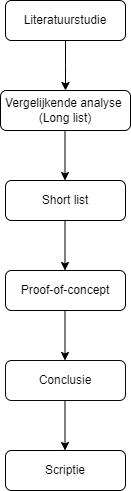
\includegraphics[width=.3\linewidth]{Flowchart.png}
    \caption{Flowchart methodologie.}
    \label{fig:Flowchart}
\end{figure}


%---------- Verwachte resultaten ----------------------------------------------
\section{Verwacht resultaat, conclusie}%
\label{sec:verwachte_resultaten}

Na het voltooien van de vergelijkende proof-of-concept wordt er verwacht dat de Classroom Management software of proxy-serveroplossing zich als effectief resulteert, zodat de E-commerce en sociale media platforms beperkt en flexibel geactiveerd worden in een klas. De keuze voor de meest geschikte oplossing hangt af van verscheidene vereisten die de balans vormen tussen gebruiksgemak, algemene kosten en functionaliteiten. De conclusie wordt gevormd door de concrete aanbevelingen voor het flexibel beheren van E-commerce en social media platforms in een onderwijsomgeving, met als doel minimalisatie van afleiding bij studenten tijdens de schooluren.

%%---------- Andere bijlagen --------------------------------------------------
% TODO: Voeg hier eventuele andere bijlagen toe. Bv. als je deze BP voor de
% tweede keer indient, een overzicht van de verbeteringen t.o.v. het origineel.
%\input{...}

%%---------- Backmatter, referentielijst ---------------------------------------

\backmatter{}

\setlength\bibitemsep{2pt} %% Add Some space between the bibliograpy entries
\printbibliography[heading=bibintoc]

\end{document}
